%\captionsetup[subfigure]{labelformat=empty}

%\begin{tikzpicture}[zoomboxarray, zoomboxarray columns=1, zoomboxarray rows=1]
%    \node [image node] { 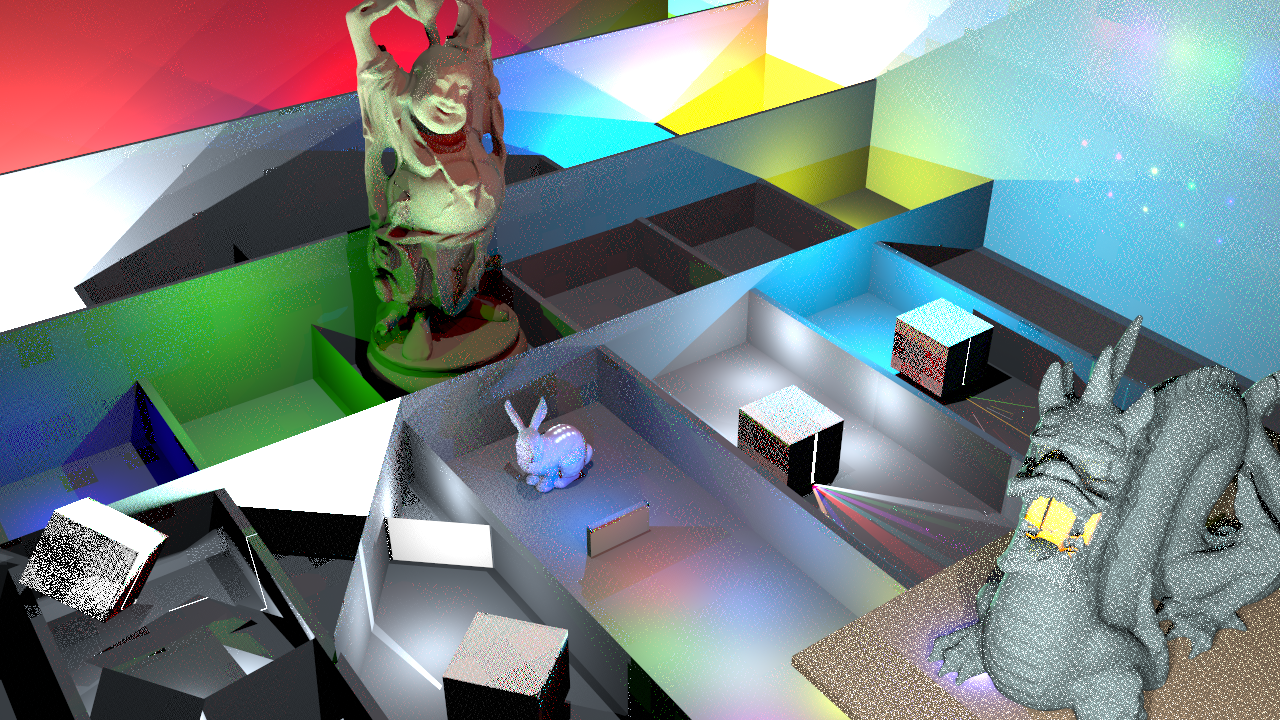
\includegraphics[width=0.5\textwidth]{figures/test2_artifacts.png} };
%    \zoombox[magnification=8,color code=yellow]{0.16,0.72}
%\end{tikzpicture}


\def\infilename{figures/test2_artifacts.png}

\newsavebox{\graph}\savebox{\graph}{\includegraphics[]{\infilename}}
\newlength\gh\setlength\gh{\heightof{\usebox\graph}}
\newlength\gw\setlength\gw{\widthof{\usebox\graph}}

\begin{scaletikzpicturetowidth}{\textwidth}
\begin{tikzpicture}[scale=\tikzscale, >=latex,
  image/.style={anchor=south west,inner sep=0}]
    \ifbool{DEBUG}{
        \node[image] (NI) at (0,0){\phantom{\usebox\graph}};
        \begin{scope}[x={(NI.south east)},y={(NI.north west)}]
            \draw[help lines,xstep=.1,ystep=.1] (0,0) grid (1.001,1.001);
            \foreach \x in {1,...,9} { \node [anchor=north] at (\x/10,0) {\x};}
            \foreach \y in {1,...,9} { \node [anchor=east] at (0,\y/10) {\y};}
        \end{scope}
    };
    \clip (0.4\gw,0.6\gh) rectangle (0.5\gw,0.7\gh);
    \node[image] {\usebox\graph};
    %\draw[|<->|,very thick,red!60] 
    %    (0.5\gw,0.5\gh) -- node[pos=0.5, auto] {$600$} ++(0.2\gw,0\gh);
\end{tikzpicture}
\end{scaletikzpicturetowidth}